\chapter{プルリクエスト --- コードレビューの文化を作る}

\section{この章で学ぶこと}

プルリクエスト（Pull Request、以下PR）は、GitHubにおけるチーム開発の中心的な仕組みです。PRは単なる「コードを統合するための手順」ではなく、チームメンバーが互いのコードを確認し合い、知識を共有し、コード品質を高めるための「場」を提供します。

オープンソースプロジェクトにおいては、見知らぬ開発者同士が安全にコードを統合するための不可欠な仕組みであり、企業のチーム開発においても、バグの早期発見や設計方針の統一のために広く採用されています。

この章では、以下の内容を学びます。

\begin{itemize}
  \item プルリクエストとは何か、なぜ必要なのか
  \item PRの作成方法（Web UI、GitHub CLI、pushと同時に）
  \item PRを構成する各要素の意味と使い方
  \item 良いPR descriptionの書き方とIssueとの連携
  \item PRのレビュー方法とsuggestion機能
  \item 3つのマージ方法の違いと使い分け
  \item ドラフトPRの活用方法
  \item PRテンプレートによるチームの運用標準化
\end{itemize}

\section{プルリクエストとは何か}

\subsection{「取り込んでほしい」という提案}

プルリクエストを一言で表現するなら、「自分のブランチで行った変更を、mainブランチに取り込んでほしい」という\textbf{提案}です。英語の「Pull Request」は「（自分の変更を）引っ張って（pull）取り込んでほしいというお願い（request）」という意味です。

この仕組みがなぜ必要なのでしょうか。仮にチームの全員がmainブランチに直接pushできるとしたら、どうなるでしょう。テストされていないコードが本番環境に入り込む、他のメンバーの変更と意図せず衝突する、いつ・誰が・なぜその変更を行ったのかが追跡しにくくなる――こうした問題が日常的に発生します。

PRを使うことで、以下の流れが実現します。

\begin{lstlisting}[language={}]
1. ブランチで開発 → 2. PRを作成 → 3. レビュー → 4. 修正 → 5. マージ
\end{lstlisting}

この流れの中で、PRは「変更を議論し、品質を確認し、合意のうえでmainに統合する」ための場として機能します。PRのページには変更の差分、コメントのやり取り、CI（自動テスト）の結果がすべて集約されるため、後から「なぜこの変更が行われたのか」を振り返ることもできます。

\subsection{なぜ直接pushしないのか}

小規模な個人プロジェクトであれば、mainブランチへの直接pushでも問題ないかもしれません。しかし、チーム開発においては、PRを経由する運用が事実上の標準となっています。その理由は以下の通りです。

\textbf{コードレビューの機会を確保するため}：他のメンバーの目を通すことで、バグの早期発見、コードの可読性向上、設計方針の統一が図れます。

\textbf{変更の意図を記録するため}：PRのdescriptionに「なぜこの変更を行ったのか」を記述することで、将来のメンテナンス時に経緯を追跡できます。

\textbf{CIによる自動テストのため}：PRの作成をトリガーにして自動テストを実行し、テストが通ったことを確認してからマージする運用が可能です。

\textbf{mainブランチの保護のため}：GitHubの「Branch protection rules」を設定すると、PRを経由しないとmainにpushできないように制限できます。

\section{PRの作成方法}

PRを作成する方法は主に3つあります。どの方法でも結果は同じですので、自分の好みやワークフローに合った方法を選んでください。

\subsection{Web UIから作成する}

最も視覚的にわかりやすい方法です。

\begin{enumerate}
  \item GitHubのリポジトリページで「\textbf{Pull requests}」タブをクリック
  \item 「\textbf{New pull request}」ボタンをクリック
  \item \textbf{base} に \cmd{main}（マージ先）、\textbf{compare} に自分の作業ブランチ（マージ元）を選択
  \item 差分が表示されるので、意図通りの変更が含まれているか確認
  \item 「\textbf{Create pull request}」ボタンをクリック
  \item タイトルとdescription（説明）を入力
  \item 必要に応じてReviewers、Labels、Linked Issuesなどを設定
  \item 「\textbf{Create pull request}」ボタンをクリックして作成完了
\end{enumerate}

\begin{figure}[htbp]
\centering
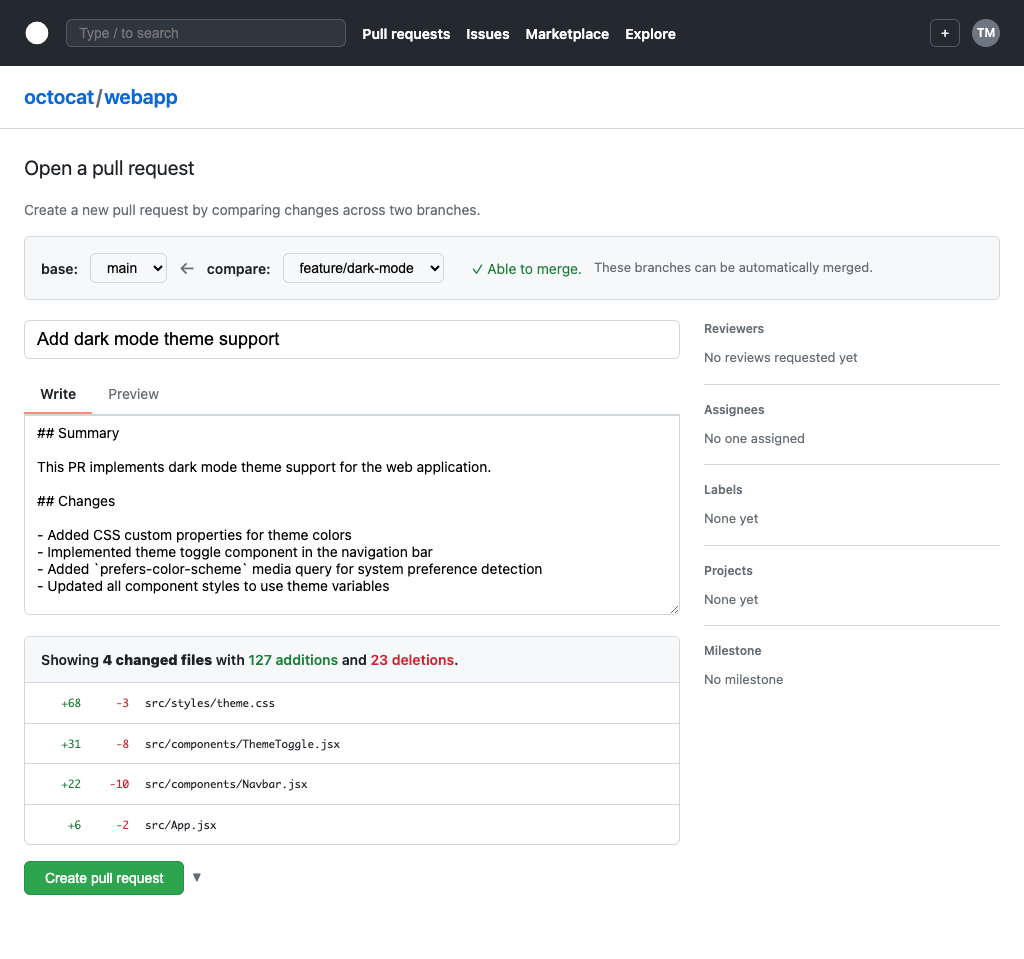
\includegraphics[width=0.95\textwidth]{images/pr-create.png}
\caption{GitHub上のPR作成画面（base、compare選択と差分表示）}
\end{figure}

この手順で重要なのは、ステップ4で差分を確認することです。意図しないファイルの変更や、デバッグ用のコードが混入していないかを、この段階でチェックしましょう。

\subsection{GitHub CLIから作成する}

コマンドライン操作が好みの方には、GitHub CLI（\cmd{gh} コマンド）を使った方法が便利です。ブラウザを開かずにターミナルからPRを作成できるため、作業の流れを中断せずに済みます。

\begin{lstlisting}[language=bash]
# 対話形式で作成する（タイトル、本文、レビュアーなどを順番に聞かれる）
gh pr create

# ワンライナーで作成する
gh pr create --title "feat: Add dark mode" --body "ダークモードを実装しました"

# ドラフトPRとして作成する
gh pr create --draft --title "WIP: New feature"

# レビュアーを指定して作成する
gh pr create --title "Fix auth bug" --reviewer alice,bob

# ラベルを付けて作成する
gh pr create --title "Fix auth bug" --label "bug,priority:high"
\end{lstlisting}

\cmd{gh pr create} を引数なしで実行すると、対話形式でタイトル、本文、レビュアーなどを入力できます。Git初心者には、まず対話形式で試してみることをお勧めします。

\subsection{pushと同時にURLを取得する}

ブランチをリモートにpushすると、GitHubがPR作成用のURLを表示してくれます。このURLをブラウザで開けば、すぐにPR作成画面にアクセスできます。

\begin{lstlisting}[language=bash]
git push -u origin feature/my-branch
# 出力にPR作成用のURLが表示される:
# remote: Create a pull request for 'feature/my-branch' on GitHub by visiting:
# remote:   https://github.com/username/repo/pull/new/feature/my-branch
\end{lstlisting}

この方法は「まずpushして、それからPRを作成する」という自然な流れに合っており、多くの開発者が日常的に使っています。

\section{PRの構成要素}

PRにはさまざまな構成要素があり、それぞれがチーム開発を円滑にするための役割を担っています。ここでは、各要素を1つずつ解説します。

\subsection{Title（タイトル）}

PRの概要を一行で表現します。チームメンバーがPR一覧を見たとき、タイトルだけで変更の内容がわかるように、簡潔かつ具体的に書きましょう。慣例として、Conventional Commits の形式（\cmd{feat:}, \cmd{fix:}, \cmd{docs:} など）を使うチームも多いです。

良い例：\cmd{feat: Add dark mode toggle to settings page}
悪い例：\cmd{Update files}（何をどう変更したのか不明）

\subsection{Description（説明）}

変更の背景、目的、具体的な変更内容、テスト方法などを記述する欄です。PRの中で最も重要な要素であり、後述の「良いPR descriptionの書き方」で詳しく解説します。

\subsection{Reviewers（レビュアー）}

PRのレビューを依頼するメンバーを指定します。指定されたメンバーには通知が届き、レビュータスクとしてダッシュボードに表示されます。チームの規模や方針によりますが、通常1〜2名のレビュアーを指定します。

\subsection{Assignees（担当者）}

PRの作業担当者を指定します。通常はPR作成者自身を設定しますが、「このPRは○○さんが引き続き対応する」といった場合に別のメンバーを指定することもあります。

\subsection{Labels（ラベル）}

PRを分類するためのタグです。\cmd{bug}、\cmd{enhancement}、\cmd{documentation}、\cmd{breaking change} などのラベルを付けることで、PRの種類を一目で識別できます。ラベルはリポジトリの Settings から自由に作成・カスタマイズできます。

\subsection{Projects（プロジェクト）}

GitHub Projectsのボードにリンクするための設定です。プロジェクト管理をGitHub Projectsで行っている場合、PRを特定のプロジェクトボードに紐づけることで、進捗状況を一元管理できます。

\subsection{Milestone（マイルストーン）}

リリース計画やスプリントに対応するマイルストーンを指定します。「v2.0リリース」「Sprint 3」などのマイルストーンにPRを紐づけることで、リリースに含まれる変更を把握しやすくなります。

\subsection{Linked Issues（関連Issue）}

PRがどのIssue（課題）を解決するものなのかを紐づけます。これは非常に重要な機能で、次節で詳しく解説するように、特定のキーワードを使うことでPRのマージ時にIssueを自動的にクローズすることもできます。

\section{良いPR descriptionの書き方}

PR descriptionは、レビュアーが変更の意図を理解し、効率的にレビューを行うための最も重要な手がかりです。コードの差分だけでは「何が変わったか」はわかっても、「なぜ変えたのか」「どういう判断でこの実装にしたのか」はわかりません。そうした情報を言語化して伝えるのが、descriptionの役割です。

\subsection{良いdescriptionの構成例}

\begin{lstlisting}[language={}]
## 概要
ユーザー認証機能を実装しました。

## 背景・目的
Issue #42 で報告されたとおり、現在のアプリケーションにはユーザー認証の仕組みが
ありません。本PRでは、JWTベースの認証機構を導入し、保護されたエンドポイントへの
不正アクセスを防止します。

## 変更内容
- JWT ベースの認証ミドルウェアを追加 (`src/middleware/auth.js`)
- ログイン/ログアウト API エンドポイント (`src/routes/auth.js`)
- パスワードハッシュ化に bcrypt を採用
- 認証関連のユニットテストを追加（カバレッジ 92%）

## テスト方法
1. `npm test` で全テスト通過を確認
2. `POST /api/login` に正しい認証情報を送信し、JWTが返ることを確認
3. 不正なトークンで保護されたエンドポイントにアクセスし、401が返ることを確認

## スクリーンショット
（UIの変更がある場合に添付）

## 関連Issue
Closes #42
\end{lstlisting}

\subsection{Issueとの連携 --- 自動クローズ}

PR descriptionに特定のキーワードとIssue番号を記述すると、そのPRがマージされたタイミングで対応するIssueが自動的にクローズされます。手動でIssueをクローズする手間が省けるだけでなく、「このPRによってこのIssueが解決された」という関連性が明確に記録されます。

使用できるキーワードは以下の通りです。

\begin{lstlisting}[language={}]
Closes #42
Fixes #42
Resolves #42
\end{lstlisting}

いずれも同じ効果ですが、バグ修正の場合は \cmd{Fixes}、機能要望の対応は \cmd{Closes} や \cmd{Resolves} を使うのが慣例です。複数のIssueを一度にクローズすることも可能です。

\begin{lstlisting}[language={}]
Closes #42, Closes #43
\end{lstlisting}

descriptionの本文中であればどこに書いても有効ですが、わかりやすさのために「関連Issue」セクションを設けてまとめて記述するのがお勧めです。

\section{PRの確認とレビュー}

PRが作成されたら、レビュアーは変更内容を確認してフィードバックを行います。GitHubのWebインターフェースには、コードレビューを効率的に行うための機能が豊富に用意されています。

\subsection{Files changedタブの使い方}

PRページの「\textbf{Files changed}」タブをクリックすると、変更されたすべてのファイルの差分が表示されます。追加された行は緑色、削除された行は赤色で色分けされるため、視覚的に変更箇所を把握できます。

\begin{figure}[htbp]
\centering
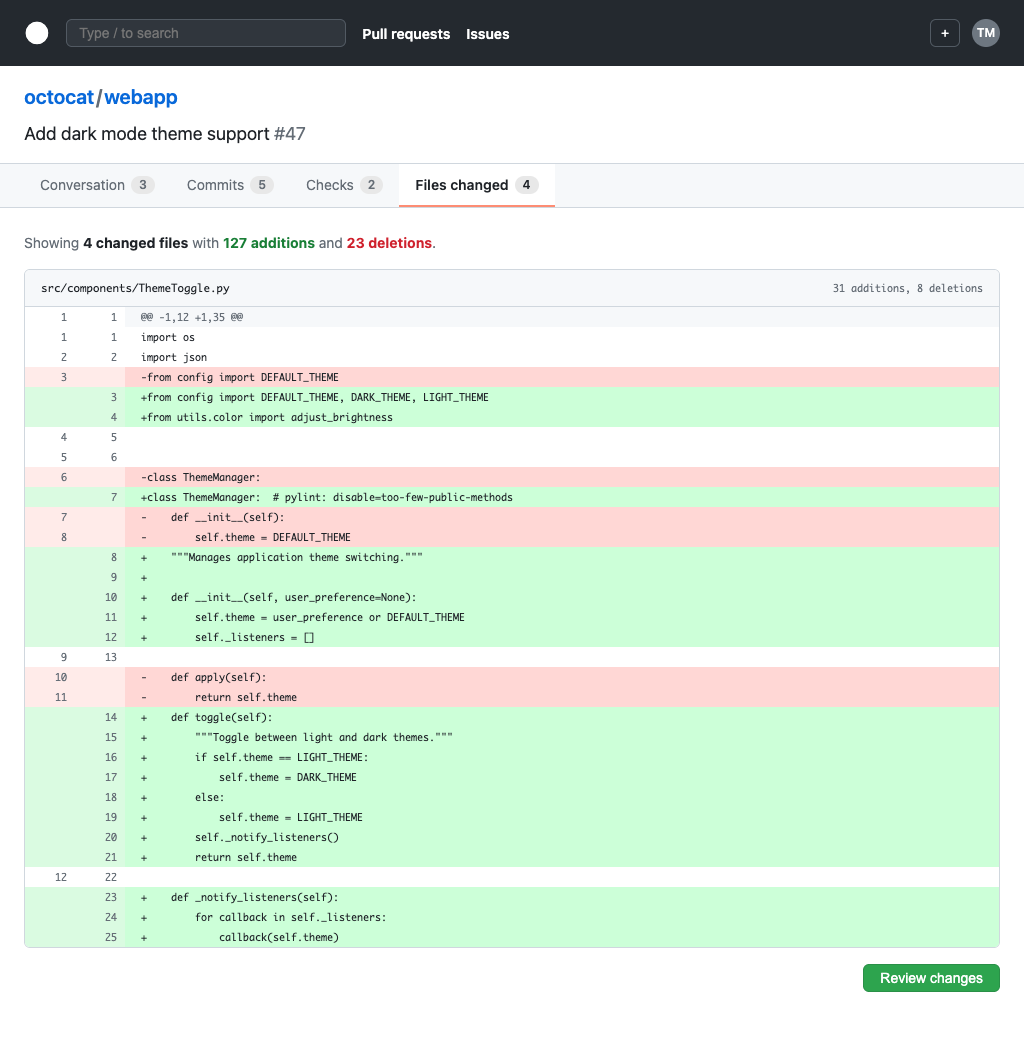
\includegraphics[width=0.95\textwidth]{images/pr-files-changed.png}
\caption{Files changedタブの差分表示画面}
\end{figure}

差分の表示方法は、「Unified（統合表示）」と「Split（左右分割表示）」の2種類から選べます。Unifiedは変更前と変更後が上下に並んで表示され、Splitは画面左に変更前、右に変更後が表示されます。好みに応じて切り替えてください。

\subsection{コメントの付け方}

特定の行にコメントを付けるには、その行の行番号の左にある「+」ボタンをクリックします。コメント入力欄が表示されるので、質問、提案、指摘などを記述できます。複数行にまたがるコメントを付けたい場合は、行番号をドラッグして範囲を選択してから「+」をクリックします。

コメントには通常のMarkdownが使えるので、コードブロックやリスト、リンクなどを自由に使って、わかりやすいフィードバックを心がけましょう。

\subsection{suggestion機能 --- 修正提案をその場で}

GitHubのレビューコメントでは、\textbf{suggestion}機能を使ってコードの修正を直接提案できます。レビュアーが「こう書き換えた方がよい」と思った場合に、言葉で説明するだけでなく、実際のコード修正案を提示できる非常に便利な機能です。

コメント入力欄で以下の形式を使います。

\begin{lstlisting}[language={}]
```suggestion
const result = items.filter(item => item.isActive);
```
\end{lstlisting}

PR作成者は、この提案を「Apply suggestion」ボタンひとつで適用できます。わざわざローカルでファイルを編集してコミット・pushする必要がないため、軽微な修正に最適です。複数のsuggestionをまとめて「Batch changes」として一度にコミットすることもできます。

\subsection{レビューの3つのステータス}

すべてのファイルを確認し終わったら、「\textbf{Review changes}」ボタンをクリックして、レビュー全体のステータスを選択します。

\textbf{Comment（コメント）}：特に承認や修正要求をせず、コメントだけを残します。軽い確認や質問のみの場合に使います。

\textbf{Approve（承認）}：変更に問題がないことを確認し、マージを承認します。リポジトリの設定によっては、一定数のApproveが得られないとマージできないように制限を設けることもできます。

\textbf{Request changes（修正を要求）}：変更に問題がある場合に、修正を求めます。修正が完了して再度レビューを受けるまで、マージがブロックされます（設定による）。

\begin{figure}[htbp]
\centering
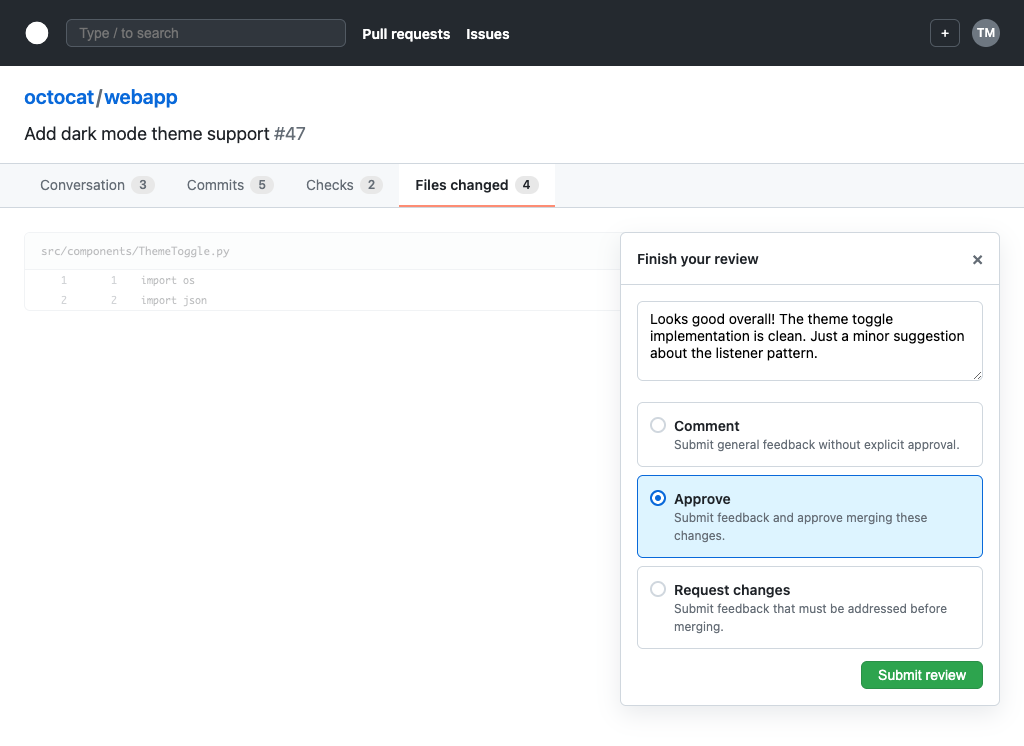
\includegraphics[width=0.95\textwidth]{images/pr-review.png}
\caption{レビュー送信時の3つのステータス選択画面}
\end{figure}

\subsection{CLIでのレビュー確認}

レビューの確認はコマンドラインからも行えます。

\begin{lstlisting}[language=bash]
# PRの一覧を表示する
gh pr list

# 特定のPRの詳細を表示する
gh pr view 42

# PRの差分を表示する
gh pr diff 42

# ブラウザでPRを開く
gh pr view 42 --web

# PRのブランチをローカルにチェックアウトして動作確認する
gh pr checkout 42
\end{lstlisting}

特に \cmd{gh pr checkout 42} は、レビュー対象のPRをローカル環境で実際に動かして動作確認する際に欠かせないコマンドです。差分を読むだけではわからないUIの挙動やパフォーマンスの問題を発見できます。

\section{3つのマージ方法}

PRの内容に問題がなく、レビューが承認されたら、いよいよmainブランチにマージします。GitHubでは3つのマージ方法が用意されており、それぞれ異なる履歴構造を生み出します。チームの方針や状況に応じて使い分けましょう。

\subsection{Create a merge commit（マージコミット）}

これはGitの標準的なマージ方法です。featureブランチの全コミットを保持しつつ、マージコミットと呼ばれる特別なコミットを作成してmainブランチに統合します。

\begin{lstlisting}[language={}]
main:    A → B → C ──────────→ M (マージコミット)
                  \            /
feature:           D → E → F →
\end{lstlisting}

\textbf{特徴}：ブランチの分岐・統合の歴史がそのまま残るため、「このfeatureブランチではどんな作業が行われたか」を後から追跡しやすくなります。一方で、featureブランチが多い大規模プロジェクトでは、履歴のグラフが複雑になりがちです。

\textbf{向いている場面}：ブランチの経緯を詳細に残したいプロジェクト、大きなfeatureの統合。

\subsection{Squash and merge（スカッシュマージ）}

featureブランチ上のすべてのコミットを1つのコミットにまとめて（squash）、mainブランチに追加します。

\begin{lstlisting}[language={}]
main:    A → B → C → DEF (D+E+Fが1つのコミットにまとまる)
\end{lstlisting}

\textbf{特徴}：featureブランチ上での細かいコミット（「WIP」「typo修正」「レビュー対応」など）がmainの履歴に表示されないため、mainブランチの履歴が非常にきれいになります。1つのPRが1つのコミットとして記録されるので、\cmd{git log} でmainの履歴を追いやすくなります。

\textbf{向いている場面}：mainブランチの履歴をきれいに保ちたい場合、featureブランチに細かいWIPコミットが多い場合。多くのチームでこの方法がデフォルトとして採用されています。

\subsection{Rebase and merge（リベースマージ）}

featureブランチのコミットをリベースしてmainブランチの先端に直線的に追加します。マージコミットは作成されません。

\begin{lstlisting}[language={}]
main:    A → B → C → D' → E' → F'
\end{lstlisting}

\textbf{特徴}：featureブランチの各コミットが個別にmainの履歴に残りますが、マージコミットが存在しないため、完全に直線的な履歴になります。各コミットのハッシュは変更されます（\cmd{D} が \cmd{D'} になる）。

\textbf{向いている場面}：各コミットが意味のある単位で整理されている場合、直線的な履歴を好むプロジェクト。

\subsection{3つの方法の比較}

\begin{tabular}{|l|l|l|l|}
\hline
\textbf{方法} & \textbf{mainの履歴} & \textbf{元コミットの保持} & \textbf{マージコミット} \\
\hline
Merge commit & 分岐・統合が残る & 全て残る & あり \\
\hline
Squash and merge & 直線的（1PR = 1コミット） & まとまる & なし \\
\hline
Rebase and merge & 直線的（個別コミット） & 個別に残る（ハッシュ変更） & なし \\
\hline
\end{tabular}

\subsection{CLIでのマージ}

\begin{lstlisting}[language=bash]
# マージコミットで統合する
gh pr merge 42 --merge

# スカッシュマージで統合する
gh pr merge 42 --squash

# リベースマージで統合する
gh pr merge 42 --rebase

# マージ後にリモートのfeatureブランチを削除する
gh pr merge 42 --squash --delete-branch
\end{lstlisting}

\cmd{--delete-branch} オプションは、マージ後に不要になったfeatureブランチをリモートから自動削除してくれます。ブランチが溜まって管理が煩雑になるのを防ぐため、積極的に使うことをお勧めします。

\section{ドラフトPR}

\subsection{ドラフトPRとは}

ドラフトPR（Draft Pull Request）は、「まだレビュー準備ができていないが、作業の進捗をチームに共有したい」場合に使うPRの形態です。通常のPRとは異なり、ドラフトPRは以下の特徴を持ちます。

\begin{itemize}
  \item PRページに「Draft」というラベルが表示される
  \item マージボタンが無効化され、誤ってマージされることを防ぐ
  \item レビュアーへの通知は送られるが、正式なレビュー依頼とは区別される
\end{itemize}

\subsection{どんな場面で使うのか}

\textbf{早期フィードバックの取得}：実装の方向性が正しいかどうかを、完成前の段階でチームメンバーに確認してもらいたい場合に使います。「この設計方針で進めてよいか」というレベルの相談ができます。

\textbf{進捗の可視化}：長期間にわたる機能開発の場合、途中経過をドラフトPRとして公開することで、チームが進捗を把握できます。

\textbf{CI/CDの事前確認}：ドラフトPRでもCIは実行されるため、テストが通るかどうかを早い段階で確認できます。

\subsection{作成と解除}

\begin{lstlisting}[language=bash]
# ドラフトPRを作成する
gh pr create --draft --title "WIP: New authentication system"

# ドラフトを解除してレビュー準備完了とする
gh pr ready 42
\end{lstlisting}

\begin{figure}[htbp]
\centering
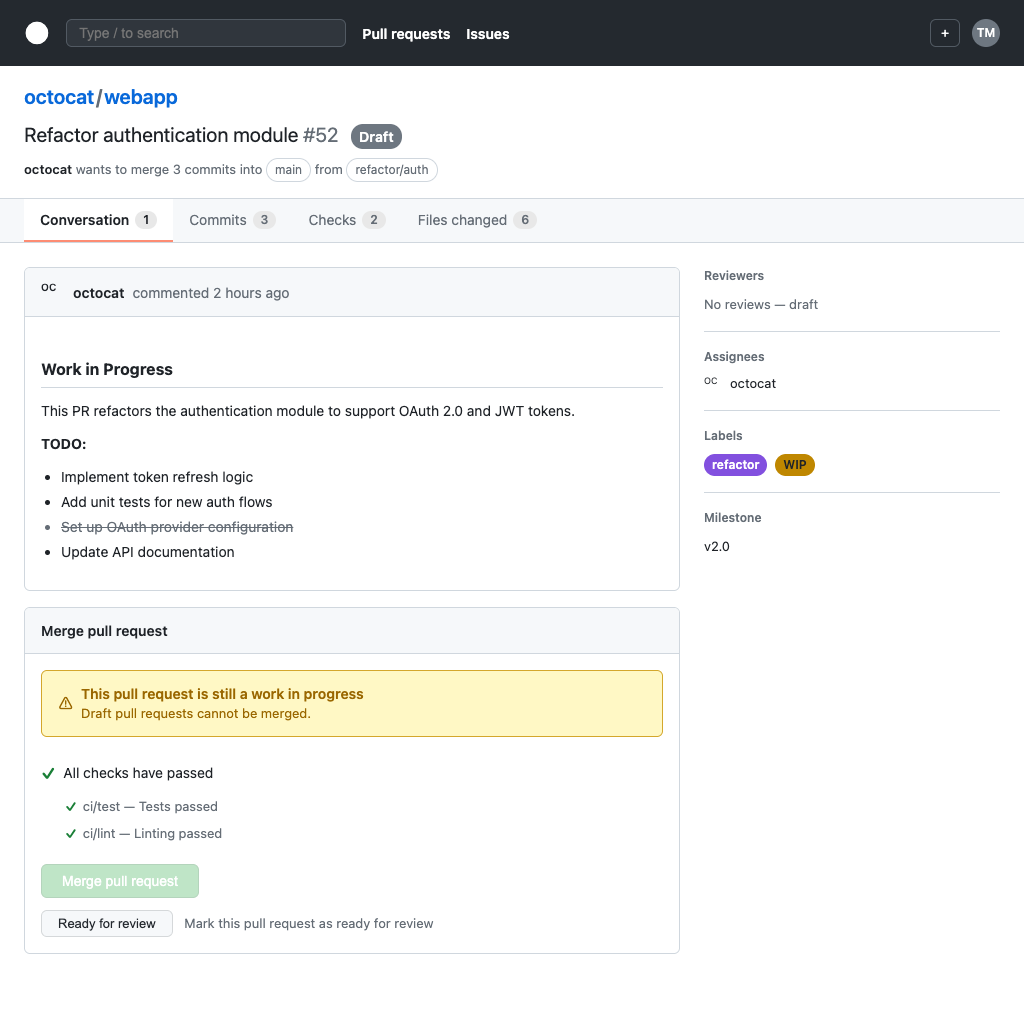
\includegraphics[width=0.95\textwidth]{images/pr-draft.png}
\caption{ドラフトPRの表示（Draftラベルとマージ不可の状態）}
\end{figure}

Web UIからは、PR作成時に「Create pull request」ボタンのプルダウンメニューから「Create draft pull request」を選択します。ドラフトPRを正式なPRに変更するには、PRページ下部の「Ready for review」ボタンをクリックします。

\section{PRテンプレート}

\subsection{テンプレートの目的}

チームで多くのPRが作成されると、descriptionの品質にばらつきが出ることがあります。「概要だけで詳細がない」「テスト方法が書かれていない」「関連Issueが紐づけられていない」といった問題が頻発すると、レビューの効率が低下します。

PRテンプレートは、PR作成時にdescription欄に自動的に挿入されるテンプレートです。チームで統一したフォーマットを用意しておくことで、全員が必要な情報を漏れなく記述できるようになります。

\subsection{テンプレートの作成方法}

リポジトリのルートまたは \cmd{.github} ディレクトリに \cmd{pull\_request\_template.md} というファイルを作成します。

\begin{lstlisting}[language=bash]
# .github ディレクトリを作成（なければ）
mkdir -p .github

# テンプレートファイルを作成
touch .github/pull_request_template.md
\end{lstlisting}

以下は、実用的なテンプレートの例です。

\begin{lstlisting}[language={}]
<!-- .github/pull_request_template.md -->

## 概要
<!-- 変更の概要を簡潔に書いてください -->

## 背景・目的
<!-- なぜこの変更が必要なのかを説明してください -->

## 変更の種類
- [ ] バグ修正
- [ ] 新機能
- [ ] 破壊的変更（既存の機能に影響がある変更）
- [ ] ドキュメント更新
- [ ] リファクタリング（機能に影響のないコード改善）

## 変更内容の詳細
<!-- 具体的に何をどう変更したかを記述してください -->

## テスト方法
<!-- レビュアーがこの変更を検証するための手順を書いてください -->
1.
2.
3.

## スクリーンショット
<!-- UIの変更がある場合は、変更前と変更後のスクリーンショットを添付してください -->

## チェックリスト
- [ ] テストを追加/更新した
- [ ] ドキュメントを更新した（必要な場合）
- [ ] セルフレビューを行った
- [ ] 動作確認を行った

## 関連Issue
<!-- Closes #XX のように記述してください -->
\end{lstlisting}

このテンプレートファイルをリポジトリにコミットしておくと、以降のPR作成時にdescription欄にテンプレートの内容が自動的に挿入されます。PR作成者は、各セクションの指示に従って内容を埋めていくだけで、必要な情報が網羅されたdescriptionが完成します。

\subsection{テンプレートの運用Tips}

テンプレートはチームの成長に合わせて改善していくものです。最初から完璧なテンプレートを作ろうとするよりも、実際に運用しながら「この情報が足りない」「このセクションは不要」といったフィードバックを反映して、徐々にブラッシュアップしていくのが現実的です。

また、テンプレートが長すぎると記入が面倒になり、形骸化してしまうリスクがあります。チームにとって本当に必要な情報に絞り、適度な長さに保つことを心がけましょう。

\section{まとめ}

この章では、GitHubにおけるチーム開発の中心的な仕組みであるプルリクエストについて、作成から運用までを包括的に学びました。

PRは「自分の変更をmainに取り込んでほしい」という提案であり、コードレビュー、議論、CIテストの場として機能します。Web UIとGitHub CLIの両方から作成でき、Title、Description、Reviewers、Labels、Linked Issuesなどの構成要素を適切に設定することで、レビュアーに必要な情報を過不足なく伝えられます。

descriptionでは「Closes \#42」のようなキーワードを使ってIssueと連携させ、マージ時に自動クローズする仕組みを活用しましょう。レビューでは、Files changedタブでの差分確認、行単位のコメント、suggestion機能を使った具体的なコード修正の提案が可能です。

マージ方法は3種類あり、Merge commit（分岐の履歴を残す）、Squash and merge（1つのコミットにまとめる）、Rebase and merge（直線的に並べる）から、チームの方針に合ったものを選択してください。多くのチームではSquash and mergeが好まれています。

さらに、ドラフトPRを活用して早期フィードバックを得る方法、PRテンプレートを使ってチーム内のdescription品質を標準化する方法も紹介しました。

PRは単なる技術的な仕組みではなく、チームのコミュニケーションツールでもあります。良いPRを書き、丁寧にレビューし合う文化を築くことが、プロジェクト全体の品質とチームの成長につながります。
